%% Requires fithesis2 module (can be downloaded from
%% https://github.com/arax/fithesis2
%% Load document class fithesis2
%% {10pt, 11pt, 12pt}
%% {draft, final}
%% {oneside, twoside}
%% {onecolumn, twocolumn}
%% sudo yum install texlive texlive-babel-czech texlive-hyphen-czech 
 
\documentclass[10pt,final,oneside]{fithesis2}
\pdfoptionpdfminorversion 7

%% Basic packages
\usepackage[czech]{babel}
\usepackage{cmap}
\usepackage[T1]{fontenc}
\usepackage{lmodern}
\usepackage[utf8]{inputenc}
\usepackage{graphicx}

%% Additional packages for colors, advanced
%% formatting options, etc.
\usepackage{color}
\usepackage{microtype}
\usepackage{url}
\usepackage{cslatexquotes}
\usepackage{fancyvrb}
\usepackage[small,bf]{caption}
\usepackage[plainpages=false,pdfpagelabels,unicode]{hyperref}
\usepackage[all]{hypcap}
\usepackage{amssymb}
\usepackage{courier}
\usepackage{listings}
\usepackage{pdfpages}

%% Fix long URLs in DVIs
\usepackage{ifpdf}

\ifpdf
\else
  \usepackage{breakurl}
\fi

%% Packages used to generate various lists
\usepackage{makeidx}
\makeindex

\usepackage[acronym]{glossaries}
\makeglossaries

\newacronym{rest}{REST}{REpresentationl State Tranfer}

\newacronym{eu}{EU}{Evropská Unie}

\newacronym{cors}{CORS}{Cross-origin Resource Sharing}

\newacronym{is}{IS}{Informační systém}

\newacronym{muni}{MUNI}{Masarykova Univerzita}

\newacronym{rdp}{RDP}{Remote Desktop Protocol}

\newglossaryentry{service-oriented-design}{
  name=service-oriented design, 
  description={lalalaa}
}

\newglossaryentry{sla}{
  name=Service-Layer Agreement, 
  description={lalala}
}

\newglossaryentry{api}{ 
  name=API, 
  description={Aplikační rozhraní (API z anglického \emph{Application Programming Interface}) označuje rozhraní poskytované k integraci programů třetích stran}
}

\newglossaryentry{resource-based-model} {
  name=resource-based model, 
  description={lalala}
}

\newglossaryentry{json}{
  name=JSON,
  description={Průběžná integrace (CI z anglického \emph{Continuous Integration}) označuje souhrn nástrojů použitých k průběžné kontrole zdrojového kódu. Typicky sem patří spouštění testů, kontrola kvality kódu, statická analýza kódu a podobně}
}

\newglossaryentry{cms}{ 
  name=CMS, 
  description={Systém pro správu obsahu (CMS z anglického \emph{Content Management System}) označuje typicky internetovou aplikaci umožňující uživatelům úpravu obsahu. Bývá také označován jako redakční systém}
}

\newglossaryentry{css}{ 
  name=CSS, 
  description={Kaskádové styly (CSS z anglického \emph{Cascading Style Sheets}) je jazyk určený k popisu vzhledu webových stránek}
}

\newglossaryentry{cvs}{
  name=CVS,
  description={Systém ke správě verzí projektu (CVS z anglického \emph{Concurrent Version System}) slouží k ukládání historie verzí zdrojového kódu}
}

\newglossaryentry{deployment}{
  name=nasazení,
  description={Proces instalace projektu na typicky vzdálený server a spuštění případných migračních skriptů a pododbně}
}

\newglossaryentry{framework}{
  name=framework,
  description={Označení pro nástroj ulehčující vývoj software, typicky obsahující podpůrné knihovny, nástroje či popisující správný postup vývoje}
}

\newglossaryentry{mediaqueries}{
  name=@Media-Queries,
  description={Pravidla jazyka CSS umožňující podmínit použití vnořených pravidel dle určíté podmínky (typicky rozlišení monitoru a podobně)}
}

\newglossaryentry{opensource}{
  name=open-source,
  description={Software jehož zdrojový kód je volně dostupný a dle licence i upravitelný}
}

\newglossaryentry{responsive}{
  name=responsivní web design, 
  description={Způsob stylování webových dokumentů, při kterém je brán ohled na různá rozlišení klientských zařízení (telefon, tablet, počítač)}
}

\newglossaryentry{servlet}{
  name=Servlet,
  description={Program v jazyce JAVA, který na straně serveru zpracovává HTTP požadavky}
}

\newglossaryentry{ssh}{
  name=SSH,
  description={Zabezpečený komunikační protokol (z anglického \emph{Secure Shell} používaný v TCP/IP sítích}
}

\newglossaryentry{wysiwyg}{
  name=WYSIWYG, 
  description={Zkratka anglického \emph{,,What you see is what you get''}, doslowně přeloženo jako ,,dostaneš to co vidíš''. Používá se pro označení editorů html kódu, které poskytují formátování pomocí tlačítek a výstup automaticky konvertují do html kódu}
}

\newglossaryentry{url}{
  name=URL,
  description={Jednotný lokátor zdrojů (URL z anglického \emph{Uniform Resource Locator} označuje řetězec znaků definující jedinečné umístění}
}

\newglossaryentry{ruby} {
  name=Ruby, 
  description={}
}

\newglossaryentry{session} {
  name=relace,
  description={Také jako sezení, označuje přetrvávající spojení mezi serverem a klientem}
}

\newglossaryentry{uco} {
  name=UČO, 
  description={Unikátní číslo studenta či zaměstnance vysoké školy}
}

\newglossaryentry{xss} {
  name=XSS, 
  description={Využití bezpečnostních chyb stránky (XSS z anglického \emph{Cross-Site Scripting} za pomoci narušení skriptů stránek a podstrčení změněného kódu či dat}
}


%% Use STAR and CIRCLE signs for nested
%% itemized lists
\renewcommand{\labelitemii}{$\star$}
\renewcommand{\labelitemiii}{$\circ$}

%% Title page information
\thesistitle{Service-oriented architecture versioning analysis and application in corporate environment}
\thesissubtitle{Diploma thesis}
\thesisstudent{Ivana Haraslínová}
\thesiswoman{false} %% Important when using Slovak or Czech lang
\thesisfaculty{fi}  %% {fi, eco, law, sci, fsps, phil, ped, med, fss}
\thesislang{en}     %% {en, sk, cs}
\thesisyear{2014}
\thesisadvisor{Ing. Leonard Walletzký, Ph.D}

%% Beginning of the document
\begin{document}

%% Front page with a logo and basic thesis information
\FrontMatter
\ThesisTitlePage


%% Thesis declaration (required)
\begin{ThesisDeclaration}
  \DeclarationText
  \AdvisorName
\end{ThesisDeclaration}

%%\chapter*{Zadání práce}
%%

\begin{ThesisThanks}

\end{ThesisThanks}

\begin{ThesisAbstract}

\end{ThesisAbstract}

%% Keywords (required)git
\begin{ThesisKeyWords}

\end{ThesisKeyWords}

%% Beginning of the thesis itself
\MainMatter

%% TOC (required)
\tableofcontents

%% Thesis text structured using
%% chapters, sections, subsections, etc.
\chapter{Introduction}
\label{chap:introduction}

Service-oriented architecture is popular architectural approach to application development. The requirements on the market are dynamically changing. Applications with service-orientation has properties which better response to the needs of market. They are flexible and have a big amount of modern technologies to be applied to their development. Service-oriented applications consist of layers where one of them contains services. They provide functionality to consumer. The consumer is in layer above and is using the services similarly as any customer which is asking for a service in real world.

Companies oriented this way offer their application as a product. Product can be consumed by more than one customer. Corresponding to the needs of each of the clients implies modifications of application to suit all of requirements. Customers can ask for changes on used application and service provider have to correspond to their requirements. Large-scale changes can have impact on all other customers so the can't be reflected immediately on application. Here origins the challenge of versioning. Versioning strategies and approaches are wide topic. There are many of them, many ideas and applications which are already in use by companies. Some services are versioned having good strategy and some of them are less good. But it can be sait that there is no universal solution how versioning should be done. 

\section{Summary}

This thesis is concerned with the services as one of the layers of service-oriented application. Specially it focuses on versioning of the services and analysis of versioning implementation in corporate environment. 

Second chapter contains a short introduction to service-oriented computing. It is a hierarchically highest concept involving service-oriented architecture, design and other principles. The service-oriented architecture (SOA) is described in more detail. There are its specifications and advantages. Further in chapter there is a section about services as a main element of SOA. There are descriptions of what they are and how are created.

Third chapter deals with the Representational State Transfer (REST). An architectural styles according which services can be designed. REST has its constraints and services has to be designed properly to be RESTful. In the chapter there is a description how to meet REST requirements. REST is composed by a set of elements are enumerated and defined. And finally there is an example of REST service.

Next chapter talks about the versioning of services - what causes a need to create a new version and how the services are versioned. There is a description of versioning strategy. The strategical decisions are done before the services are developed. During the versioning the strategy is applied. There are many approaches to version, two of them are analyzed in detail.

Chapter five is about the versioning access. Provider can make the services available by various approaches. The concrete techniques are listed with their examples and applications on REST services. There is a summary of advantages and disadvantages based on the opinion of experienced programmers. At the end of chapter is a table with example of version access of well-known REST services.

Sixth chapter analyzes and apply the versioning on a real company. It introduces a company's architecture and talk about the versioning strategy. It design a possible evolution and changes within their services.

%What are the services will be described in first part. There is ,. The service oriented architecture (SOA) is described in more detail. %Services are components of the SOA. 


\chapter{Service-oriented computing}
\label{chap:service-oriented computing}
\emph{Service-oriented computing} represents a distributed computing platform. [1] It has its own paradigm, logic, architecture and patterns. It is built on the distributed computing platforms and extends it by new considerations about governance, design layers and technologies suitable for its implementation.
\emph{Service orientation} is a design paradigm, it divides the system into logic units which are separately shaped and can be utilized according to strategic goals and benefits of a requested result.

\section{Service-oriented architecture}
\emph{Service-oriented architecture (SOA)} is a set of best practices for an organization leading to agile architectural model of the system to meet business needs. Result of applied practices is an architecture which corresponds to dynamic market changes. The SOA best practices are describing the human behaviour, there is no list of constraints which have to be followed to obtain a service-oriented architecture. The best practices are designed to resolve specific situations which the organization can meet and depending on them could be selected just a subset of appropriate practices which are necessary to apply.

One of the main advantages of a service-oriented architectural style is its ability to efficiently deal with changes. SOA is based on a decomposition of enterprise IT assets and separation of "stable" IT artifacts (services) from "changeable" artifacts (business processes), orchestrating services into IT solutions (processes) \cite{website:versioning-in-soa}. %(http://msdn.microsoft.com/en-us/library/bb491124.aspx)
The speed of changes in the bussines department is too fast to be passed directly into development and maintance of the monolitic systems. Funcionality of this systems is designed on measure of customer and can't deal easily with changes, often it is needed to interfere in design of whole architecture. SOA offers better support when the business requirements change, the changes are refleted into modification of an existing business process, or if it's needed a new process is created using existing services \ref{sec:services}. There are more approaches how to deal with the changes and one of them is versioning \ref{chap:versioning}.


\section{Services}
\label{sec:services}
Services are the logic units form which is composed the \gls{service-oriented-design}. Every service is standalone object or component. Every service has its own functional context and related capabilities. Each service is deployerd independetly on another one and on the system which use it. It allows the parallel development, one service can be the part of many products of the corporation.
The essence of Service in the SOA context is the business abstraction - that is a representation of funcionality and/or data presented in business context.[Agile architecture].

\subsection{Levels of service} 

There are three levels of how we can interpret the expression \emph{'Service'} in SOA context \cite{agile-architecture}:
\begin{enumerate}
  \item \textbf{Service implementation} \hfill \\
Service implementation is the code performing the logic.
  \item \textbf{Service interface} \hfill \\ 
This level is an entry point to the sevice implmentation, it provides underlying logic to consumers but encapsulating it in a way that consumers can see the implementation. 
  \item \textbf{Abstracted service} \hfill \\
Abstracted service or business service represents a business capability or data. This services can be composed to describe a business process. This is a core abstraction of SOA.
\end{enumerate}

There is a many-to-many relationship between these three entities. Business service can represents muliple interfaces and in the same time one interface can be supported by multiple implementation.

/TODO image

\subsection{Service categories and types} %(http://msdn.microsoft.com/en-us/library/bb491121.aspx)

There are two main types of services. The first type is composed by infrastructural services which provide the facilities and aren't a part of application. To the second type belongs services which are the part of the application and provide main logic.

/TODO decribe services

\begin{description}
  \item[Bus services] can be further divided into 
  \begin{enumerate}
    \item Communication services 
    \item Utility services
  \end{enumerate}
  \item[Application services] consist of   
  \begin{enumerate}
    \item Entity services
    \item Capability services
    \item Activity services
    \item Process services
  \end{enumerate}
\end{description}

/TODO image

\section{Services granularity}
During the analytical part of the service design it can be defined the service granularity. The service granularity describes functional scope of the serivce. When the granularity is fine, it means the service contains little logic. On the other hand there are coarse-grained serices which have complex logic but at the expense of flexibility.
Defining the granularity can help to determine the characteristics of the serivce - its performance or size of message. \cite{soa-contract}S

\section{Approaches to implementation}

\subsection{Evolution of approches}
\subsubsection{WSDL RPC SOAP} 
/TODO form agile arcitecture revolution
 
\subsection{REST}
/TODO WADL

Representational State Transfer, REST is an architectural style for building ditributed hypermedia applications.
Thanks to REST disappeared many issues related to web services, but it comes with some new. This thesis deals with REST style and RESTfull services. \ref{chap:rest}

%%\subsubsection*{\textbf{Guacamole} \hfill \emph{http://guac-dev.org/}}
%%\label{subsec:guacamole}
%% \ref{}.
%%    \item \textbf{[název předmětu 1]} \hfill \\
%%    odkaz na stránku předmětu, obsahující pouze název a informace o spolufinancování \gls{eu}
    
%%\begin{table}
%%  \caption{Základní typy entit v Drupalu}
  %%\label{tab:typy-entit}
  %%\begin{tabular}{ | p{3cm} | l | c | c | }
   %% \hline 
    %%Typ entity & Strojový název & Dostupnost polí & Rozšiřitelnost \\ \hline 
    %%Komentář & comment & \checkmark & \checkmark \\ \hline 
    %%Soubor & file &  & \\ \hline 
    %%Slovník & vocabulary &  & \\ \hline 
    %%Uzel & node & \checkmark & \checkmark \\ \hline 
    %%Uživatel & user & \checkmark & \checkmark \\ \hline 
    %%Záznam slovníku & term & \checkmark & \checkmark \\ \hline             
  %%\end{tabular}
%%\end{table}
%% \emph \emph \texttt.


\chapter{Representative State Transfer (REST)}
\label{chap:rest}

\lstset{frame=none,
  language=JAVA,
  aboveskip=3mm,
  belowskip=3mm,
  showstringspaces=false,
  columns=flexible,
  basicstyle={\small\ttfamily},
  numbers=none,
  breaklines=false,
  breakatwhitespace=false,
  tabsize=3
}

\section{REST architecture}
\label{sec:rest-architecture}

REST is "a set of constraints on the overall architectural approach" \cite{agile-architecture}. Roy Thomas Fielding described REST in his doctoral dissertation as an architectural style. The constraints are applied to obtain desired properties of developed architecture. REST is applicable to \gls{hypermedia} applications where multimedia nodes are connected via hyperlinks.

REST architecture is client-server. The server holds implemented logic of services and encapsulates it under the interfaces. The interfaces are entry points for client. Through them data can be obtained and modified. 

\begin{figure}[htp] \centering{
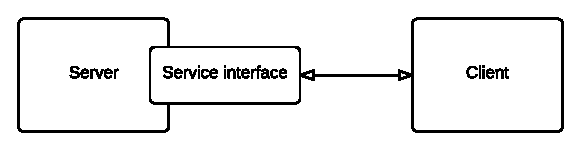
\includegraphics[width=8cm]{img/communication-through-interface.pdf}}
\caption{Client enter the server through the interfaces}
\label{fig:communication-through-interface}
\end{figure} 


The REST is \gls{resource-based-model}. It operates resources named by nouns and actions are provided by HTTP requests. 
REST architecture is a composition of \emph{elements}, \emph{connectors} and \emph{components}. None of them defines specific technology, they are abstractions. The elements abstract a behaviour of components. The components have their roles, the way of interaction among them and interpretation. The REST coposition will be described in Section \ref{sec:rest-composition}

REST has its best practices and constraints. Only services which are built according to this definition can be called \emph{RESTful}. Six constraints characterizing the REST will be described further in Section \ref{sec:constraints}.

\section{Composition of REST}
\label{sec:rest-composition}
As was mentioned above, REST architectional style consist of data elements, connectors and components, shown in Figure \ref{fig:composition-rest}. REST is resource-based, so the main data element is a resource. It is accompanied by resource metadata. Next elemetns are represenatation and its metadata. The last set od data elements are control data. Other than elements REST consists of connectors and components.

\begin{figure}[htp] \centering{
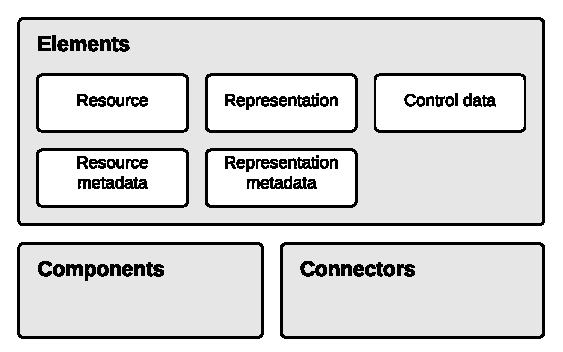
\includegraphics[width=8cm]{img/composition-rest.pdf}}
\caption{Composition of REST}
\label{fig:composition-rest}
\end{figure} 

\subsection{Data elements}
\subsubsection{Resource}
  Resource is an abstraction of information. Any information which can be named by noun can be a resource. "A resource is a conceptual mapping to a set of entities.." \cite{fielding} or set of values. The values can be resource identifiers and representations.
  Resource can be static (for example \emph{an image}) or dynamic (\emph{the time} which dynamically changes).
  
  Examples:
  \begin{center} 
  \begin{lstlisting}
      customer, 
      account, 
      order, 
      ..
  \end{lstlisting} 
  \end{center}

\subsubsection{Resource identifier}
  Serves to identify resources. The resource identifier is assigning a name thanks to which it is possible to reference appropriate resource. The identifier is \gls{url}. It marks a path to reach the resource. A request from client is routed to the specific service and method.
It should be possible to perform the \gls{CRUD} operations with the resources, every operation can be mapped on HTTP method. Having the method and the path the specific operation is performed.

Examples: \\
\begin{center}
\begin{tabular}{l l l}
Method & URL Path & Operation performed \\ \hline
GET & /customers & Retrieves all customers \\
GET & /customers/5 & Retrieves customer with id 5 \\
POST & /customers & Creates new customer \\
PUT & /customers/13 & Updates customer with id 13 \\
DELETE & /customer/2 & Deletes customer with id 2 \\
\end{tabular}
\end{center}

\subsubsection{Representation}
  Representation is used by REST components to perform changes to the resource. The representation stands for a part of (less commonly the whole) resource state. Format of representation's data is called media type and affects the performance of the \gls{hypermedia}. Media types can be proprietary or standardized, from standardized types. There are for comparison \gls{xml} and \gls{json}. JSON format is less verbose and smaller than XML and in consequence in sake of data transmission it would perform faster than a XML representation format.
  
Example of representation:
\begin{center}
  \begin{tabular}[b]{l l}
    In XML format & \begin{lstlisting}
    <?xml version="1.0" encoding="utf-8">
    <customer> 
      <name>Peter<\name> 
      <surname>Smith<\surname> 
      <dateofbirth>20-4-1975<\dateofbirth> 
    <\customer>
    \end{lstlisting} \\
    
\\
    
    In JSON format & \begin{lstlisting}
    {
        "name": "Peter", 
        "surrname": "Smith", 
        "dateofbirth": "20-4-1975"
    }
    \end{lstlisting}
  \end{tabular}
\end{center}

\subsubsection{Representation metadata}
  Representation metadata describes the data of which the representation consists. For example Content-Type defines the \gls{mime-types} of representation sent between client and server. Last-Modified defines the date of last modification of requested object.

  \begin{center}
  \begin{lstlisting}
    {Content-Type: application/json}
    {Content-Type: application/xml}
    {Last-Modified: Thu, 19 May 2015 21:58:55 GMT}
    
  \end{lstlisting}
  \end{center}
  
\subsubsection{Resource metadata}
  Resource metadata describes resources. The examples are Vary which comunicate with proxies whether use a cashed response or request a new ono. Other example is Allow. It defines the allowed methods for a specified resource.
  
  \begin{center}
  \begin{lstlisting}
    {Vary: *}
    {Allow: GET}
  \end{lstlisting}
  \end{center}
  
\subsubsection{Control data}
  "Control data defines the purpose of a message between components, such as the action being requested or the meaning of a response." \cite{fielding}. It can control the caching and parametrize requests. An example can be If-Modified-Since which allows to return a specified response message (304 Not Modified)
  
  \begin{center}
  \begin{lstlisting}
    {If-Modified-Since: Thu, 16 Jun 2014 20:31:00 GMT}
  \end{lstlisting}
  \end{center}
  
  

To summarize the REST elements, every resource has its representation which describes how are resources manipulated in RESTful \gls{api} architecture. The representation is a part or whole resource state. It is transferred between the client and server and has generaly JSON or XML format, but could be in many other formats as well. Representations and resources have their metadata which describe them. Control data affects the messages between client and server.

Client sends a message to server when he wants to operate with a resource. This message is a request. It contains a resource identifier which locates the resource. The request has headers filled by metadata describing the resource and representation. And the body of request involves a representation. An example of a request to create a new customer.

Request:
\begin{center}
  \begin{lstlisting}
     POST /cutomer HTTP/1.1
     Content-Type: application/json
     If-Modified-Since: Thu, 16 Jun 2014 20:31:00 GMT

     {
        "name": "Peter", 
        "surrname": "Smith", 
        "dateofbirth": "20-4-1975"
     }
  \end{lstlisting}
  \end{center}
  
Response:
  \begin{center}
  \begin{lstlisting}
     HTTP/1.1 200 OK 
     Content-Type: application/json
     Allow: POST
     
     {
        "id": 23, 
     }
  \end{lstlisting}
  \end{center}
  
     
The client want to save a representation of customer to the resources. Resources are accessed by URL. Headers are consisting of representation content type which is JSON and control data of modification since specified date. The response message contains headers with content type of a representation and method which is allowed by resource metadata. The response returned an id of created customer. 





\subsection{Connectors}
The connectors encapsulate transfer of representations and access of resources. Connectors are: client, server, cache, resolver, tunnel. %TODO explanation, maybe image

\subsection{Components}
REST components are an abstraction of application unit. The components are origin server, gateway, proxy, user agent. %TODO explanation, maybe image

\section{REST constraints}
\label{sec:constraints}

The REST architectural style has to be developed with respect to its constraints. They are applied to an architecture to create RESTful services. This rules leads to desirable properties of the system, such as performance, scalability, simplicity, modifiability, visibility, portability and reliability. Constraints described below were defined by Roy Thomas Fielding and there are six of them in total.
%%(citacia http://www.restapitutorial.com/lessons/whatisrest.html#)
 
%TODO write about HATEOAS

\subsection{Uniform Interface}
  
Interface stands between client and server. Through the interface client access the server. The REST interface is uniform, client and server always use a fixed set of methods to provide operation over the resources. REST uses \emph{\gls{http} specification}, mostly GET, POST, PUT and DELETE verbs. Despite REST can work with other protocols and define different verbs it uses HTTP operations for practical purpposes. This concept than separates client and server allowing them to develop each part independently and to reduce the coupling between them. %The interface is uniform, so that is easy to understand for both, the server and the client.

Interface is resource-based. Resources are on the server side and the client sents a request process either create, get, update or delete operation over the resource. The request contains a resource identifier in \gls{uri}. It identifies a path to concrete resource. Depending on the type of the request, represention is sent from the client in request and/or from the server in response. The representation is conceptually separated from the resource. It represents appropriate database record.

Resources are manipulated exclusively through the representations. The representation with any metadata attached keeps enough information to modify the resource on the server.

%Sent message represents a clients request or a servers response and it is self-descriptive. It means there is enough information to know how to process the message and the response explicitly defines the cashability.

The representation is sent in a request using HTTP verbs (GET, POST, PUT, DELETE,..) and the URI. Server sends to the client a HTTP response. For illustration a simplified HTTP request and response format is shown in Figure \ref{fig:http}.

\begin{figure}[htp] \centering{
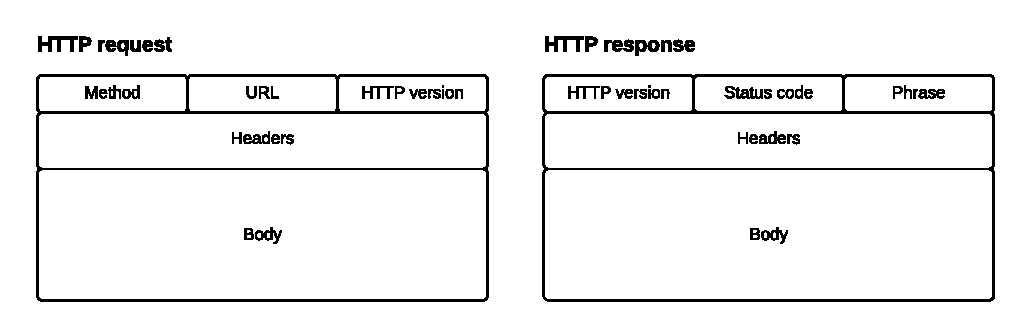
\includegraphics[width=12cm]{img/HTTP.pdf}}
\caption{HTTP request and response}
\label{fig:http}
\end{figure} 

Firts line in the request is called request line. It contains a name of method to be executed over the resource, the URL and HTTP version to be used. Then there are headers and the body for a representation. The response has the fist line starting with HTTP version, than there is a status code with appropriate phrase. Status and phrase reporting whether the request was successful or not.

\subsection{Stateless}
  
Each message is self-descriptive. Request has enough context to be understood and the messages have no state. Any state of a \gls{session} is held just on the client side (for example a logged-in user's session).
The statelessness allows greater scalability, because server doesn't have to communicate with the session, which can be created to carry the state using another architectural style of services. Reliability is improved because of easier recovery of partial failures. Disadvantage is that the sent requests contain repetitive data and the server has lower control over the application's behaviour.

\subsection{Client-server}

RESTful architecture is client-server oriented. There are two separate concerns. It is properly defined what is consumer's side and what are services on server side. Client can’t have direct access to the database, assets or resources. Client-server architecture improves portability of both client and server codes because they are standing alone. The architecture provide simplicity and scalability of server-side code because it doestn't have to include user interface. Client and server are linked together thanks to unified interface and the two can be developed independently.

\subsection{Cacheable}

Server responses (representations) are cacheable. They can be stored to eliminate the interactions with server . Responses can be defined as cashable implicitly, explicitly or negotiated. The cache can be established on server-side, client-side or both as can be seen on Figure \ref{fig:cacheability}. The reason for caching is to reduce interactions over the network. Cached responses are loaded from the cache instead of sending a request to the server. 
Cacheing partially decreses the client-server interaction but improves the scalability and performance. 


\begin{figure}[htp] \centering{
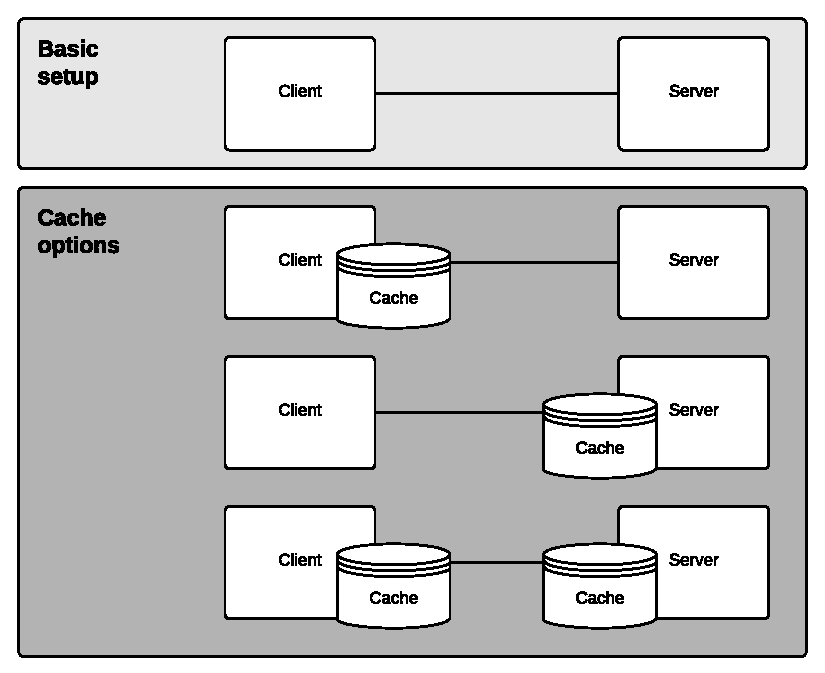
\includegraphics[width=10cm]{img/cacheablity.pdf}}
\caption{Cacheability options}
\label{fig:cacheability}
\end{figure} 

\subsection{Layered system}

This constraint is linked to cashability and client-server principle. System is composed of layers which rapresent independent parts of the system. Example of vertically layered system is shown on Figure \ref{fig:layered-system}. Client is not able to see whether he is communicating directly with the server, or with an intermedia between them. Intermedia improves scalability, provide shared caches and moreover can enforce security policies.

\begin{figure}[htp] \centering{
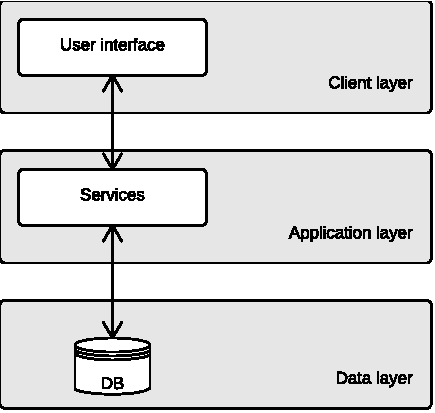
\includegraphics[width=7cm]{img/layered-system.pdf}}
\caption{Layered system example}
\label{fig:layered-system}
\end{figure} 

\subsection{Code on demand}

The logic can be transferred to the client-side. This way the server can temporarily extend or customize the functionality of the client. This can be performed for example by the components like service-side scripts.
This constraint is unique, it is the only one which can be violated and the services can be still RESTful.

\section{Application of REST}

Having the SOA and knowing the constraints of the REST services can be designed. When a company wants to develop a system with RESTful services it has to apply at least the first five of constraints. But it can occur that not all the constraints are profitable for an application. In this case the architecture can forget some of them but the services cannot be further marked as RESTful. This notation doesn't affect services themselves, the result can be still the best design for current application. The RESTful services and their constraints are one of the possible resolutions of architectural style. They are not the universal solution for system architecture.

\subsection{RESTful service example}
There is a corporation with SOA and its services are designed according to REST constraints. One of the services is representing business abstraction of \emph{customers} of the company. Customers can be viewed, created, modified or deleted. The HTTP verbs (GET, POST, PUT, DELETE) are used to perform the operations. 

In designing the service there is considered the notation of \gls{webapi} \gls{framework}. 

Resource identifier is a \gls{uri} address. ASP.NET Web API is composed of \emph{controller} and an \emph{action}. The controller is a class handling the HTTP request and the action is a method of the controller. In this example the controller is \emph{customers}, the action can be \emph{GET} and to identify a specific customer the parameter \emph{name} as to be a part of URI.

\begin{lstlisting}
    GET     customers/getByName/{name} 
\end{lstlisting}

When the client wants to get the customer whose name is \emph{Peter} then the request looks like:

\begin{lstlisting}
    GET     customers/getByName/Peter 
\end{lstlisting}

Thanks to URI the request is routed to specific resource and returns a response. In this response is a representation containing customer identified by requested name. Representation has its media type which are stated in the metadata in this  example it's JSON format:

\begin{lstlisting}
    { 
    "name": "Peter",
    "surname": "Sun",
    "e-mail": "peter.sun@service.com" 
    }
\end{lstlisting}

When the number of customers increases it is not hard to realize that the name identifier is not sufficient. There might be more than just one of the customer named "Peter". The name is obviously not unique and the best solution how to identify an entity is to assign it unique \emph{id} identifier. 

The request and response than look like:
\begin{lstlisting}
    GET     customers/getByName/{id} 
    
    GET     customers/getByName/2 
    
    { 
    "id": 2,
    "name": "Peter",
    "surname": "Sun",
    "e-mail": "peter.sun@service.com" 
    }
\end{lstlisting}


In case the service from the example above is already released and used by client a change can be done. The need of changes like this one is seriously affecting server and client and it is necessary the change is implemented by both of them. How to handle them is a main topic of this thesis and will be explained and analyzed in the rest of this work.

\chapter{Versioning}
\label{chap:versioning}

Versioning determines creation of releases of a product and its management. The product is what provider offers to consumer. A new version of product is created when a modification is needed. Consumers can use the same product but they can use its different version. The version could have been released because of new requirements or due to improvements of functionality. 

Any of new versions of the product mustn't influence the execution of consumers code. When the product is customized, a change has to be compatible with all consumers. In case the change is incompatible, it is needed to release a new version. Before a consumer switches the new version an agreement between provider and consumer has to be established. The consumer has to do required changes within his functionality deriving from the new agreement.

A change which leads to necessity of modification on consumer side can be a new requirement from one of the consumers, the new version is released and the consumer can immediately switch to use it. Other consumers can follow their schedule and switch to the newest version when it is suitable for them. 

In service oriented architecture the product are services as they are descibed in section \ref{sec:services}. Provider is one who provide services, server. Consumer is one who use services, client.

\section{Version compatibility}
\label{sec:v-compat}
There are two forms of versioning concerning compatibility. \cite{website:service-versioning}
\begin{description}
  \item[Compatible changes] \hfill \\
  Compatible changes are that changes of product which do not harm any consumer. Compatible changes are for example implementation bug fixes or change in number of parameters in interface to support an implementation modification.
  \begin{enumerate}
    \item[Backward compatible] \hfill \\ 
  When a new version of a service is deployed the consumer of an earlier version must be capable to interoperate with the new version without any modification of his application. If a service is backward compatible it is compatible with older version of itself. Backward compatible change can be an addition of a new resource or a new capability to the resource. \hfill \\ 
  Example: \hfill \\ 
  Service has capability \hfill \\ 
  \begin{lstlisting}
  GET   /customers/{customerId}
  \end{lstlisting}
  and we add a new capability to get only the name of a customer with assigned id
  \begin{lstlisting}
  GET   /customers/{customerId}/name
  \end{lstlisting}

  This addition doesn't harm any consumer of the service, because they can continue to use every capability which has been already integrated in their systems. Every capability is still a part of the new version of the service. 
  
  \item[Forward compatible] \hfill \\
  The service version is forward compatible when it is designed in a way it can support future modifications. The newer version of service can be deployed without influence on its usability by consumers. 
  \end{enumerate}
  
  \item[Incompatible changes] \hfill \\
  Incompatible changes are breaking changes which affect consumers of services. An example is removal of an action or change of types or order of parameters of an action.
  \begin{enumerate} 
    \item[Backward incompatible changes]  \hfill \\
    Backward incompatible changes are changes which break the consumers using an earlier version of service. It means that the new version is no longer backward compatible and do not interpret the data of its earlier version.
    \item[Forward incompatible changes] \hfill \\
    These changes break the forward compatibility of the service. It means that a future version won't be compatible with existing one, any modifications of current version don't preserve compatibility.
  \end{enumerate}
\end{description}

\section{Versioning of services}
\label{sec:verioningservices}
Thanks to versioning services can be evolved and customized. When a breaking change of a service occurs the new version can be created so that existing consumers of services are not affected. Release of a new version doesn't harm the previous one, all versions can coexist and be used at the same time. 

\subsection{Versioning on different levels of a service}
As there are three levels of interpretation of a \emph{service} as was already described in section \ref{subsec:levels-of-service}. A change and consequent creating of a new version can occur within each of this levels - business abstraction, service interface and service implementation.

\subsubsection{\textbf{Versioning of service implementation}}
The implementation of a service can be changed. The new version of service is backward compatible or backward incompatible. The backward compatible modification in this level is simple bug fix, the incompatible changes are changes which affect the interface of the service. This type of versioning is elucidate in section \ref{sec:implversioning}

\subsubsection{\textbf{Versioning of service interface}}
As mentioned service interface is an entry point for consumers to work with the services. Interface can be versioned as well and its change has impact on the consumer application. Compatible changes of the interface are for example addition of an action on the other side non compatible change is removal of an operation. When a new action is added no one is using it and it is optional if somebody would make use of it. When an action is removed, consumers which have used it are broken. How to version an interface is explained in section \ref{sec:interfaceversioning}

\subsubsection{\textbf{Versioning of business service}}
Sometimes it is needed to change the business service. It means the business which is abstracted have to be changed. For example because of new requirements due to legislative a business service needs modifications, if this kind of change affects behaviour, semantic or functionality modification of existing service it is easier to create a new service rather than a version. 

\section{Service implementation versioning}
\label{sec:implversioning}
The implementation is encapsulated under the interface and it is not visible for outer world. Despite this the implementation cannot be replaced without affecting the whole service. A provider of service has a contract including \gls{sla} with a service consumer. The contract has to be followed because it is valid document on which the consumer relies. 

Every change which has to be done in the implementation of the service needs to be validated against the contract. When the implementation which is going to be replaced is the breaking change from the point of view of the consumer the agreement with the change of contract is needed and consequently the new version has to be released.

Changes of the implementation lead to the versioning of the code. Compatible changes can be done without necessity of new version, but they can be versioned after specific amount of changes (this amount should be specified as a parto of SOA governance as a part of versioning strategy, see section \ref{sec:version-strategy}), just for proper change management. In case of a breaking change, the code has to be versioned. Incompatible changes requires \gls{deprecation}, code which has been changed needs to be deprecated to not break the consumer's code. Deprecation ensures the backward compatibility of changes.

%popis infrasturkury
Lets have a company which has two streams, one where a development proceed and the other one is a staging stream with stable code. At this point the code is versioned, the version in the company can have a format \{stream name\}\{version number\}. Code present in the staging stream is possible to build and produce the dll files. Dll files are deployed on a server. Consumers are connecting to this server to use services. The process can be seen at the Figure \ref{fig:soa-architecture}
%TODO add dll in glossary, add stable in glossary

\begin{figure}[htp] \centering{
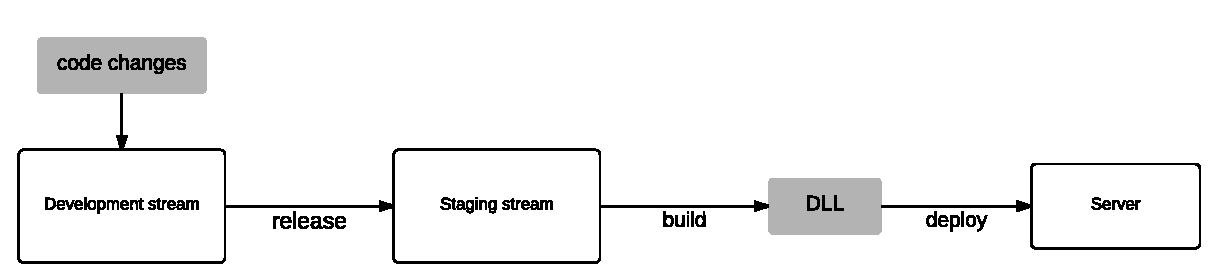
\includegraphics[width=13cm]{img/service-implementation.pdf}}
\caption{Process of deployment of implementation changes}
\label{fig:service-implementation}
\end{figure} 

\bigskip

On the server is just one version of the code. If another version is needed to be available it has to be deployed on another server. Then customers are using different servers, as shown on the image \ref{fig:consumer-server}

/TODO unfinished section

\begin{figure}[htp] \centering{
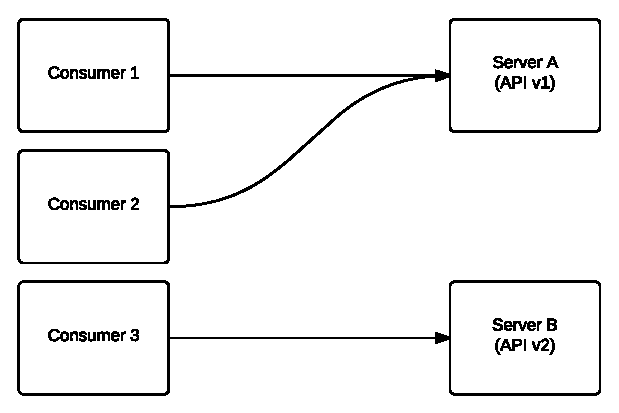
\includegraphics[width=10cm]{img/consumer-server.pdf}}
\caption{}
\label{fig:consumer-server}
\end{figure} 

\section{Service interface versioning}
\label{sec:interfaceversioning}

The service layer of an application which is developed by provider is composed of projects containing services. These services represent the service interface as the access point for consumer. Services contains methods (actions) which ensure operations over the services. The design is shown on Figure \ref{fig:service-layer-design}

\begin{figure}[htp] \centering{
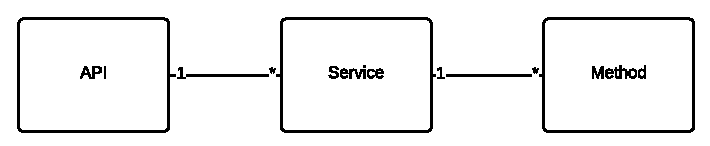
\includegraphics[width=11cm]{img/service-layer-design.pdf}}
\caption{Design of service layer}
\label{fig:service-layer-design}
\end{figure} 

This interpretation of service versioning is the most interesting for the analysis and brings various approaches. The versioning of services is quite young topic and there are still very vibrant discussions of the best approach. The analysis is executed in chapter \ref{chap:versionaccess}.

%Each version has its own implementation and is distinguishably addressed.

TODO unfinished

%Versioning management of services requires the proper definition of following concepts \cite{website:versioning-in-soa}:
%what will be versioned and how, the life-cycle of the versions and the access to the version.
%\begin{enumerate}
 % \item Units of versioning
 % \item Service changes, constituting a new version
 % \item Service version life-cycle considerations
 % \item Version deployment/access approaches
%\end{enumerate}

\section{Versioning strategy}
\label{sec:version-strategy}
There is a need to specify a set of rules to version services consistently. This rules form the versioning strategy. They are related to release of a new version of services or number of services which should be active at the same time. The rules are the matter of SOA governance. There isn't single correct way to govern the service versioning. Defined strategies should be followed and practiced during whole service lifecycle \cite{soa-governance}:

\begin{description}
  \item[Strict] 
  Any change of a service results in a new version. This strategy does not support backward or forward compatibility.
  \item[Flexible]
  Any incompatible changes result in a new version and the service design supports backward compatibility.
  \item[Loose]
  Any incompatible changes result in a new version and the service design supports backward and forward compatibility.
\end{description}

\subsection{Version identifiers}
Identification of the version is one of the fundamental design patterns. Version is indicated by decimals separated by periods. The version number length and common meaning of the digits should be established as a part of the versioning strategy. Every digit increments releatively to significance of the change. It is usually composed from two to four digits X.Y.Z.R.

Explanation of the digits \cite{soa-governance}:

\begin{enumerate}
  \item[Major changes X] \hfill \\
  Major changes are non-backward compatible changes, after a major change the new document schema is no longer compatible with the old one. These changes break the usage of the service by the consumer. They are imposed to the new version and consumers need to adjust their programs to switch to this version. Breaking changes can be performed by adding or removing an enumeration, removing or renaming a global type or element, changing the optionality of an element from optional to required.
  
    \item[Minor changes Y] \hfill \\
  Minor changes are backward-compatible changes. The changes do not impact consumers, the new version continue to support the consumers working with the old version. Examples can be new optional element to existing type, a change of optionality of a local element from required or optional, adding global type or global element, etc.
  
  \item[Patch version Z] \hfill \\  
  Patch version Z is incremented if only backwards compatible bug fixes are introduced. A bug fix is defined as an internal change that fixes incorrect behavior.
  
  \item[Revisions R] \hfill \\  
  Revisions are changes without semantic content, for example formatting, comments, etc. They do not affect the functionality of the service and service consumers.
\end{enumerate} 

Using version identifiers to express the compatibility by incrementing major and minor numbers serve to compatibility guarantee. There is another approach to indicate the version of services related to amount of work. The number increment according to effort which have been dedicated to the change. The big effort increments the major number and modest effort the minor number. This two approaches can be combined and in most cases they are, preserving mainly the compatibility guarantee and less often communicating the effort made. \cite{soa-governance}


\subsection{Service version life-cycle}
Service life-cycle defines the time period in which a version should be maintained. When the time is short, customers have not enough time for their upgrades required in order to switch on new verion. On the other hand when the period is too long, too many versions of service have to be maintained. The suitable time span is a result of consideration of individual organization with respect to their capability to deal with changes.

Product version should be always compatible with consumers usage. When a new version of the service method is released, it is needed to have the old one present in the implementation if any of the consumers operate with it. When the service method is going to be replaced by new one, it has to be held so that do not impact any consumer. It can be signed as deprecated, which do not influence its usage from the point of view of the consumer, but it means that provider waits that all consumers switch to the new implementation. When the deprecated method stops to be used, it can be safely removed. 

This lifecycle is possible only when the service method versioning approach is implemented, in case of whole-service versioning, when the service is given into state deprecated, it is equivalent to its remove, it is needed the new agreement between the provider and consumer so that consumer have to implement changes to use the new service %or just keep using the older version. 
The whole-service versioning provides less flexibility.

\section{Units of versioning}
It is needed to define what will be versioned. Most frequent are three possibilities, versioning of project, of services contained in project or of service methods. The relationship between this is shown in Figure \ref{fig:service-layer-design}.


\subsection{Versioning of project}
  /TODO 
\subsection{Versioning of service}
  The whole service is versioned with all its methods. This approach is working well with the object-oriented and the component-base development. It's not appropriate with coarse-grained services (\ref{sec:granularity}). \cite{website:versioning-in-soa} 
  
  This approach doesn't provide much flexibility.
  
\subsection{Versioning of service method}
  In most cases the change arises just in a method or some methods of the service. It is not necessary to version the whole service, but there is an option to version just these operations.
  The benefits of this approach are less code which is deployed because just a changed methods are redeployed in a new version. All services are immutable, their name and classification remain unchanged when there is a method added. The changes concern just a consumers which use the method, instead of consumers of the service containing changed method. 
  When the versioning of method is used it is needed to deploy each method with its own endpoint address, the advantage is that the \gls{sla} is provided for the method so that it is not changed the SLA of the same service.
  Moreover the addressing schema becomes more complex, the consumer has to specify not just the service but also the method and version of method which wants to use.
In spite of the more elaborate routing this possibility of versioning offers more flexibility. It adapts the services versioning to versioning practices of commonly used programming languages. 
Other benefit of this approach is deprecation, an old method which has new version can be signed as deprecated. The method can become deprecated when a better alternative is implemented but there are still consumers which use the old one. This method can remain in service until all consumers switch to the newest method.


%\subsection{Version definition}
%It is necessary to analyze the services/methods from the point of view of changes, their impact on the consumer. Analysis of possible changes deals with influence of change on the consumers execution and consequently defines the changes which will break it. When the change of the service or method is breaking it leads to the creation of new version.

%The components of the service are interface and message, both of them could be changed and cause the release of new version.

%\subsubsection{Interface changes}
A change of interface has significant impact on the consumer, it requires many modification of customers implementation or even completely new service. The deprecation of a method is equivalent to its removal and should occur rarely.
%When following semantic messages model, the interface is never changed. Advantage of this approach has source in the fact that all changes can be done just within the methods of service. 
When the methods are units of versioning they are deployed individually and new methods can be added without any impact on existing consumer. When the method is going to be removed, it is first deprecated, so that is still kept around the service and could be used until all consumers stop to use it. The changes are contained in messages and are not shown within the interface.
Than as seen it is better to design the versioning definition in order to not include the interface changes.



%\subsubsection{Message changes}
%When using the semantic message model the changes of service interface do not change the interface itself but are contained in message. The message is created by a schema which describes its content. Changes in schema can provide different cases of compatibility with actual implementation and can be divided in three categories:

%\subsection{Version access}
%It is needed to define how different consumers of services are accessing its version of the service. There are several approaches everyone has its pros and cons. The access possibilities are described in separate chapter \ref{chap:versionaccess}.

%\section{Versioning service implementation}
%Besides versioning the service interface, it is possible to consider an implementation. The underlying implementation can changed without affecting the interface itself. 

\chapter{Version access}
\label{chap:versionaccess}

When the service interface is versioned the client has to know how to access requested version. There are more ways to implement this functionality. It has to be part of the agreement between client and server. Producer of service creates an access point for the new version and consumer has to modify his implementation according to agreed pattern to switch to this new version. 


\section{Version identifiers}
Version is typically identified by decimal number. The number is composed from a minor and a major number. Their increase can be based on the amount of work which have been done between two releases of versions or the compatibility regarding the two versions. This approaches can be combined.

\section{Access approaches}
Deployment of the versions can be performed different ways. There are two main approaches:
\begin{enumerate}
  \item Version parameter
  \item Multiple endpoint addresses
\end{enumerate}

\subsection{Version parameter}
Every consumer of the services uses the same endpoint address to access the services. Single service has the same address for any of its implementations. Then then the object of versioning is the implementation. Behind one service which is accessed by one URI there are possibly more implementations.
To access a requested version of the implementation it's used version parameter. It is present in request message sent by consumer. Thanks to the parameter the request is routed to appropriate implementation version.

This approach is advantage for consumers, release of new version has minimal impact on them. But on the other side it requires a special attention on version strategy, it can lead to collision of names, database names, ecc.

\subsection{Multiple endpoint addresses}
In this approach each service version is deployed independently and has its own endpoint address. This time consumer is obliged to know which service and implementation versions wants to access. When a customer wants to pass to newer version he needs to make changes in request addresses. The advantage of the approach is that the names collisions are eliminated by independent deployment of service versions. But the routing is more complex and requires addressing registry for resolving the addresses.

/TODO zdroj Versioning in SOA, obrazky

There are a lots of different theories and opinions about the right approach to implementation of the versioning. The most discussed are the URI versioning and versioning using the headers. Uri versioning represents a multiple endpoint addresses approach described above and version in headers represents the version parameter approach.

\section{Versioning using URI}
Version in URI is broadly used solution how to version. The version is displayed in the URI address:

\texttt{http:/api.com/v1/accounts/123}

This approach is easy to understand. The URI change when a new version is released so that it routes to the right version. But this approach brings a lot of disadvantages. There are more option how to handle with consumers - let the consumer change the URI every time the version changes, or a consumer obtains fixed URI or the consumer can change its implementation from scratch, which does not involve many work, but it is unacceptable regarding a user.
Everyone form this option is constraining the flexibility.
The version should not influence the consumer usability of the system and has to have minimal possible impact on it. If the consumer should change the routing everytime he switch to the new version it is not good and there are possibilities how to access the version better.

Moreover having a look at the REST constraints, as they are described by Fitztadidaa, this approach violates the HATEOS principle. But there are several opinions that this principle is not going to be followed in modern service design. 
/TODO finish section 

The URI containing version can be used for internal purposes, when the code is debugged and tested, but in the production should not be present.

\section{Versioning based on headers}
\subsection{Link header}
The link header can be used to define version of the service which should be used. When the request is sent the consumer obtain a response which is enriched by the link. When consumer uses the old version of the service he just ignores the link. The user of the new service can follow the added link and reach the newest version of the response.

\texttt{http://example.com/v2/rels/v2-equivalent}

\texttt{GET /accounts/123 HTTP/1.1}

\texttt{HTTP/1.1 200 OK}
\texttt{link: <http://example.com/v2/orders/super-widget>; rel="alternate http://example.com/v2/rels/v2-equivalent"}

%\subsection{Location}

\subsection{MIME Types}

\texttt{GET /accounts/123 HTTP/1.1}

\texttt{Accept: application/vnd.v2+json}


Versioning strategies in popular REST APIs (http://www.lexicalscope.com/blog/2012/03/12/how-are-rest-apis-versioned/)
\begin{center}
\begin{tabular}{l l l}
API NAME & VERSIONING &	EXAMPLE \\
Twillo & date in URI \\
Twitter &	URI \\
Atlassian & URI \\
Google Search	& URI	\\
Github API	& URI/Media Type in v3 & Intention is to remove versioning in favour of hypermedia – \begin{lstlisting}current application/vnd.github.v3\end{lstlisting} \\
Azure	& Custom Header	& \begin{lstlisting}x-ms-version: 2011-08-18\end{lstlisting} \\
Facebook & URI/optional versioning	& \begin{lstlisting}graph.facebook.com/v1.0/me\end{lstlisting} \\
Bing Maps &	URI	\\
Netflix	& URI parameter	& \begin{lstlisting}http://api.netflix.com/catalog/titles/series/70023522?v=1.5\end{lstlisting} \\
LinkedIn &	URI &	\begin{lstlisting}http://api.linkedin.com/v1/people/~/connections\end{lstlisting} \\
Foursquare	& URI	& \begin{lstlisting} https://api.foursquare.com/v2/venues/40a55d80f964a52020f31ee3?oauth_token=XXX&v=YYYYMMDD \end{lstlisting} \\
Google data API (youtube/spreadsheets/others)	& URI parameter or custom header & \begin{lstlisting}"GData-Version: X.0" or "v=X.0" \end{lstlisting} \\
Salesforce & URI with version introspection & \begin{lstlisting}
{"label":"Winter '10"
"version":"20.0",
"url":"/services/data/v20.0",} 
\end{lstlisting} \\
PayPal &	parameter	& \&VERSION=XX.0 \\
Drop Box	& URI &	\begin{lstlisting}https://api.dropbox.com/1/oauth/request_token \end{lstlisting}\\
Youtube data API versioning &	URI	& \begin{lstlisting}https://www.googleapis.com/youtube/v3\end{lstlisting} \\
\end{tabular}
\end{center}

\chapter{Conclusion}
\label{chap:conclusion}
To understand the service versioning it is necessary to know the service-oriented architecture (SOA). It was introduced in at the beginning of the thesis. SOA works with services which were described with their relationship to real-world processes. When a company is going to produce an application or system which is service-oriented, it has to analyze the real-world processes and group them by logical units. Those units are services and especially the network operated ones were described in detail.

The thesis outlines Representational State Transfer (REST) architectural style. REST is one of the possible approaches to implementing web services. There are several concepts related to this architecture which need to be followed to obtain RESTful services. 

Versioning is an inevitable part of the service lifecycle. As the real-world changes, the requirements on applications are changing over time as well. The services has to respond to those changes. Every reaction on the change request has to be rooted in versioning strategy. The strategy should be determined during the analytical part. 

Number of approaches to version the services are quite infinite. What is important is a result - provide the service to client. The breaking change require an effort from both to integrate it independently of versioning approach. The main difference between having just one version and more distinct versions accessible at the time has two points of view. From provider side the difference is if he has to wait to client who integrates the service or whether he can deploy new version of API immediately. From client point of view, it can be said, the difference is in amount of accessible versions. 
This thesis analyze two approaches to versioning to demonstrate the differences and impact of each of them on service consumer and provider. This can be helpful to make an overview of approaches for consideration about the versioning strategy for an API. 

Another part of thesis describe consumers access the services version. The URL addresses should be permanent. This results from the REST constraint Uniform interface and connected HATEOAS aspect. After a change of the interface the new version is created. When the services specific versioning approach is used, both API can be deployed and run at the same time. These two versions has a particular way how to access them. The common techniques are enumerated. The techniques can be than further analyzed and customized for particular application. 


This thesis can be further extended several ways. The work presents only analysis of existing versioning techniques. It can be used as a base for creation a versioning strategy of API. Other extension can be deep analysis of Invest s.r.o. API in order to rework the versioning strategy of the company.  




%% Lists of tables and figures, glossary, etc.
\printindex
\printglossary[type=\acronymtype,title={Abbrevations}]
\printglossary
\listoffigures
\listoftables

%% Bibliography from references.bib
\begingroup
\def\tmpchapter{0}
\renewcommand{\chaptername}{}
\renewcommand{\thechapter}{}
%\addtocontents{toc}{\setcounter{tocdepth}{-1}}
\chapter{References}
\renewcommand{\chapter}[2]{}% for other classes

\bibliographystyle{plain}
\bibliography{iharaslinova}

%\addtocontents{toc}{\setcounter{tocdepth}{2}}
\endgroup

%% Additional materials
\appendix

%% End of the whole document
\end{document}
